\section{Block-Encodings}
\label{sec:block-encoding}

\subsection{Definition}


\subsection{Linear Combination of Unitaries}
\label{subsec:lcu}

\subsection{Sparse Block-Encoding of Pairing Hamiltonians}
\label{subsec:sparse-be}
%stuff from Liu et al
%\ws{Might ask you to fill this out @Gus}
LOBE builds off of the work of Liu et. al \cite{liu2024efficient}, which describes a sparse block-encoding structure for pairing Hamiltonians. This block-encoding has three main parts: state preparation (and state un-preparation), the select oracle, and the coefficient oracle. The general idea of these unitaries is that the \textit{select} oracle tells where the non-zero matrix elements are, while the \textit{coefficient} oracle tells what the values are of the corresponding matrix element. 
In practice, however, it is done slightly differently. The \textit{select} oracle acts on some state $\ket{\psi}$ to output a new state $\ket{\phi}$ in a way in which a term in the Hamiltonian acts, while the coefficient oracle picks up the corresponding coefficient of this term. 

The pairing Hamiltonian, in which \cite{liu2024efficient} is based on is given as 
\begin{equation}
    H = \sum_{ij}h_{ij}b^\dagger_i b_j
\end{equation}

The general layout of these circuits is as follows: 

\begin{figure}[h]
    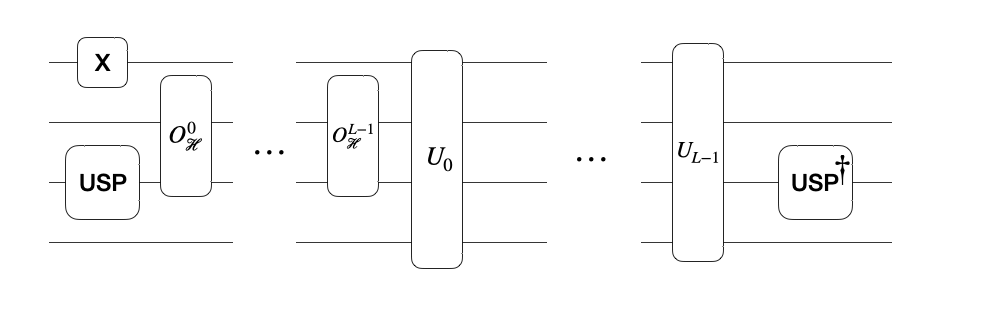
\includegraphics[width = \linewidth]{figures/SBE.png}
    \caption{Circuit for sparse block-encoding Pairing Hamiltonians}
\end{figure}

The \textit{USP} gates act similarly to the \textit{prepare} operator in LCU; however, it doesn't load information about the coefficients of the Hamiltonian terms. It simply creates an equal superposition of basis states from $\ket{0}\dots \ket{L - 1}$ where $L$ is the number of terms in the Hamiltonian. 

The $O_\mathcal{H}$ oracle is a controlled rotation on the rotation ancilla that, given the basis state from the index register, rotates the ancilla via $R_y\left(2\arccos(\alpha_l) \right)$, where $\alpha_l$ is the coefficient for the term $T_l$ in $H$. 

The \textit{select} oracle is built up of the unitaries denoted as $U_0 \dots U_{L - 1}$ which perform the action of applying the Hamiltonian on some input state. Each of the unitaries in this oracle $U_i$ encodes the behavior of one term $T_l$. In general, there are three main parts of each of these unitaries: 
\begin{enumerate}
    \item Control on index and system register. The index control will denote a particular term in the Hamiltonian while the system register will control on the system state this operator acts non-trivially on. Target on the control qubit. This qubit now becomes the control for the actual action of the Hamiltonian term.
    \item Fredkin gate to swap the occupations of the system register for $i \leftrightarrow j$. This is beecause $b^\dagger_i b_j \ket{\psi}$ is nonzero when $\ket{\psi}_i = \ket{0}$ \textit{and} $\ket{\psi}_j = \ket{1}$, in which after the term acts on $\ket{\psi}$, $\ket{\psi}_j$ and $\ket{\psi}_i$ will swap values,  \textit{or} when they are both $\ket{1}$, in which case, the operator becomes a number operator.
    \item Set validation qubit to $0$ to signify $H\ket{\psi}$ was performed. 
\end{enumerate}